%!TEX program = xelatex
\documentclass[cn,pad,11pt,epub,epubblue]{elegantnote}

\title{ElegantNote:一个优美的 \LaTeX{} 笔记模板}

\author{\href{https://ddswhu.me/}{邓东升}}
\institute{\href{https://elegantlatex.org/}{Elegant\LaTeX{} Program}}
\version{2.20}
\date{}


\begin{document}
\maketitle
% logo
\centerline{
\includegraphics[width=0.25\textwidth]{logo.pdf}}

\setlist[itemize]{label=$\circ$}

\section{模板设计}
此模板设计的初衷是为了记录笔记,在 2013 年开始构想,初版我们设计了非常美观的定理环境,并设计了 3 套不同的颜色主题。但我们发现在实际记笔记的时候,过多的定理区块使得整个文章并不是非常美观,所以我们把 ElegantNote 更新为 ElegantBook 模板,在后面被用户熟知。而 ElegantNote 的设计自此停止。

2018 年,在被一些用户“催更”之后,ElegantBook 迎来重大更新,原先浮动的定理环境用 tcolorbox 全部改写。时至今日,ElegantBook 版本为 3.05。之后,我们便想把 ElegantNote 也彻底更新下,放弃 ElegantBook 中的定理环境设计,改用更为紧凑,更加朴素的定理环境,设计更适合笔记记录和笔记阅读的 \LaTeX{} 模板。

在一些朋友的建议和启发下,我们基于标准的 \LaTeX{} 文类 article 重新设计了新版 ElegantNote 模板,在此特别感谢!新模板有下面几个特性:
\begin{itemize}
\item 添加护眼模式,颜色为绿豆沙颜色,默认为白色背景;
\item 适配不同设备,包括 Pad(默认),Kindle,PC(双页),通用(A4);
\item 5 套颜色主题,分别是:\textcolor{egreen}{green}(默认),\textcolor{ecyan}{cyan}, \textcolor{eblue}{blue}, \textcolor{sakura}{sakura}, \textcolor{black}{black};
\item 语言模式支持:中文(默认),英文;
\item 支持 \hologo{pdfLaTeX} 和 \hologo{XeLaTeX} 编译;
\item 更加美观的图表标题格式,列表环境,数学字体等。
\end{itemize}

\subsection{护眼模式}
本模板增加了护眼模式,默认为不开启,开启的方法如下:
\begin{lstlisting}[frame=none]  
\documentclass[geye]{elegantnote} % or
\documentclass[mode=geye]{elegantnote}
\end{lstlisting}

\begin{remark}
此次更新只添加了护眼模式(绿豆沙色背景),如果您有希望增加其他颜色,可以在 \href{https://github.com/ElegantLaTeX/ElegantNote}{Github::ElegantLaTeX/ElegantNote} 创建 issues 或者发邮件给我们。
\end{remark}

\subsection{设备选择}
为了让笔记方便在不同设备上阅读,免去切边,缩放等操作,本模板适配不同的屏幕大小,分别为 Pad,Kindle,PC,A4。不同屏幕的选择为
\begin{lstlisting}[frame=none]  
\documentclass[device=pad]{elegantnote}
\documentclass[device=kindle]{elegantnote}
\documentclass[device=pc]{elegantnote}
\documentclass[device=normal]{elegantnote}
\end{lstlisting}
\begin{note}
也可以采取直接赋值的方法选择屏幕,比如:
\end{note}
\begin{lstlisting}[frame=none]  
\documentclass[pad]{elegantnote}
\documentclass[kindle]{elegantnote}
\documentclass[pc]{elegantnote}
\documentclass[normal]{elegantnote}
\end{lstlisting}

\begin{note}
如果想要得到普通的 A4 纸张大小的 PDF,需要选择 \lstinline{device=normal},而不是选择 \lstinline{device=pc},因为  \lstinline{device=pc} 实际上设置的是电脑双页模式。
\end{note}

\subsection{颜色主题}
本模板内置 5 套颜色主题,分别是 \textcolor{egreen}{green},\textcolor{ecyan}{cyan}, \textcolor{eblue}{blue}, \textcolor{sakura}{sakura}, \textcolor{black}{black}。其中 green 为默认颜色主题,如果用户不需要彩色,可以选择 black 主题。颜色主题的启用方法和之前一样:
\begin{lstlisting}[frame=none]  
\documentclass[green]{elegantnote}
\documentclass[color=green]{elegantnote}
...
\documentclass[black]{elegantnote}
\documentclass[color=black]{elegantnote}
\end{lstlisting}

\subsection{语言模式}
本模板内含两套语言环境,改变语言环境会改变图表标题的引导词(图,表),文章结构词(比如目录,参考文献等),以及定理环境中的引导词(比如定理,引理等)。不同语言模式的启用如下:
\begin{lstlisting}[frame=none]  
\documentclass[cn]{elegantnote} 
\documentclass[lang=cn]{elegantnote} 
\documentclass[en]{elegantnote} 
\documentclass[lang=en]{elegantnote}
\end{lstlisting}
\begin{note}
只有中文模式才可输入中文,如果需要在英文模式下输入中文,可以自行添加 \lstinline{ctex} 宏包\footnote{需要使用 \lstinline{scheme=plain} 选项才不会把标题改为中文。}或者使用 \lstinline{xeCJK} 宏包设置字体。另外如果在笔记中使用了抄录环境(\lstinline{lstlisting}),并且其中包括了中文,请务必使用 \hologo{XeLaTeX} 编译。本说明文档也只能通过 \hologo{XeLaTeX} 编译。
\end{note}

\subsection{编译方式}

本模板支持两种编译方式,\hologo{pdfLaTeX} 和 \hologo{XeLaTeX}。模板测试环境为 Win10 + \TeX{} Live 2019。

\subsection{定理类环境}
此模板采用了 \lstinline{amsthm} 中的定理样式,使用了 4 类定理样式,所包含的环境分别为
\begin{itemize}
\item \textbf{定理类}:theorem,lemma,proposition,corollary;
\item \textbf{定义类}:definition,conjecture,example;
\item \textbf{备注类}:remark,note,case;
\item \textbf{证明类}:proof。
\end{itemize}

\begin{remark}
在选用 \lstinline{lang=cn} 时,定理类环境的引导词全部会改为中文。
\end{remark}

\section{写作示例}

我们将通过三个步骤定义可测函数的积分。首先定义非负简单函数的积分。以下设 $E$ 是 $\mathcal{R}^n$ 中的可测集。

\begin{definition}[可积性]
设 $ f(x)=\sum\limits_{i=1}^{k} a_i \chi_{A_i}(x)$ 是 $E$ 上的非负简单函数,其中 $\{A_1,A_2,\ldots$, $A_k\}$ 是 $E$ 上的一个可测分割,$a_1,a_2,\ldots,a_k$ 是非负实数。定义 $f$ 在 $E$ 上的积分为
\begin{equation}
   \label{inter}
   \int_{E} f dx = \sum_{i=1}^k a_i m(A_i).
\end{equation}
一般情况下 $0 \leq \int_{E} f dx \leq \infty$。若 $\int_{E} f dx < \infty$,则称 $f$ 在 $E$ 上可积。
\end{definition}

\begin{table}[htbp]
  \small
  \centering
  \caption{燃油效率与汽车价格}
    \begin{tabular}{lcc}
    \toprule
                    &       (1)         &        (2)      \\
    \midrule
    燃油效率        &    -238.90***     &      -49.51     \\
                    &     (53.08)       &      (86.16)    \\
    汽车重量        &                   &        1.75***  \\
                    &                   &       (0.641)   \\
    常数项          &  11,253***        &    1,946       \\
                    &  (1,171)          &   (3,597)      \\
    观测数          &      74           &       74        \\
    $R^2$           &       0.220       &        0.293    \\
    \bottomrule
    \multicolumn{3}{l}{\scriptsize 括号内为标准误} \\
    \multicolumn{3}{l}{\scriptsize *** p<0.01, ** p<0.05, * p<0.1} \\
    \end{tabular}%
  \label{tab:reg}%
\end{table}%

一个自然的问题是,Lebesgue 积分与我们所熟悉的 Riemann 积分有什么联系和区别?之后我们将详细讨论 Riemann 积分与 Lebesgue 积分的关系。这里只看一个简单的例子。设 $D(x)$ 是区间 $[0,1]$ 上的 Dirichlet 函数。即 $D(x)=\chi_{Q_0}(x)$,其中 $Q_0$ 表示 $[0,1]$ 中的有理数的全体。根据非负简单函数积分的定义,$D(x)$ 在 $[0,1]$ 上的 Lebesgue 积分为
\begin{equation}
   \label{inter2}
   \int_0^1 D(x)dx = \int_0^1 \chi_{Q_0} (x) dx = m(Q_0) = 0
\end{equation}
即 $D(x)$ 在 $[0,1]$ 上是 Lebesgue 可积的并且积分值为零。但 $D(x)$ 在 $[0,1]$ 上不是 Riemann 可积的。

\begin{theorem}[Fubini 定理]\label{thm:fubi}
若 $f(x,y)$ 是 $\mathcal{R}^p\times\mathcal{R}^q$ 上的非负可测函数,则对几乎处处的 $x\in \mathcal{R}^p$,$f(x,y)$ 作为 $y$ 的函数是 $\mathcal{R}^q$ 上的非负可测函数,$g(x)=\int_{\mathcal{R}^q}f(x,y) dy$ 是 $\mathcal{R}^p$ 上的非负可测函数。并且
\begin{equation}
   \label{eq:461}
   \int_{\mathcal{R}^p\times\mathcal{R}^q} f(x,y) dxdy=\int_{\mathcal{R}^p}\left(\int_{\mathcal{R}^q}f(x,y)dy\right)dx.
\end{equation}
\end{theorem}

公式~(\ref{eq:461}),公式~\eqref{eq:461}

\begin{proof}
Let $z$ be some element of $xH \cap yH$.  Then $z = xa$ for some $a \in H$, and $z = yb$ for some $b \in H$. If $h$ is any element of $H$ then $ah \in H$ and $a^{-1}h \in H$, since $H$ is a subgroup of $G$. But $zh = x(ah)$ and $xh = z(a^{-1}h)$ for all $h \in H$. Therefore $zH \subset xH$ and $xH \subset zH$, and thus $xH = zH$.  Similarly $yH = zH$, and thus $xH = yH$, as required.
\end{proof}

\begin{figure}[!htbp]
	\centering
	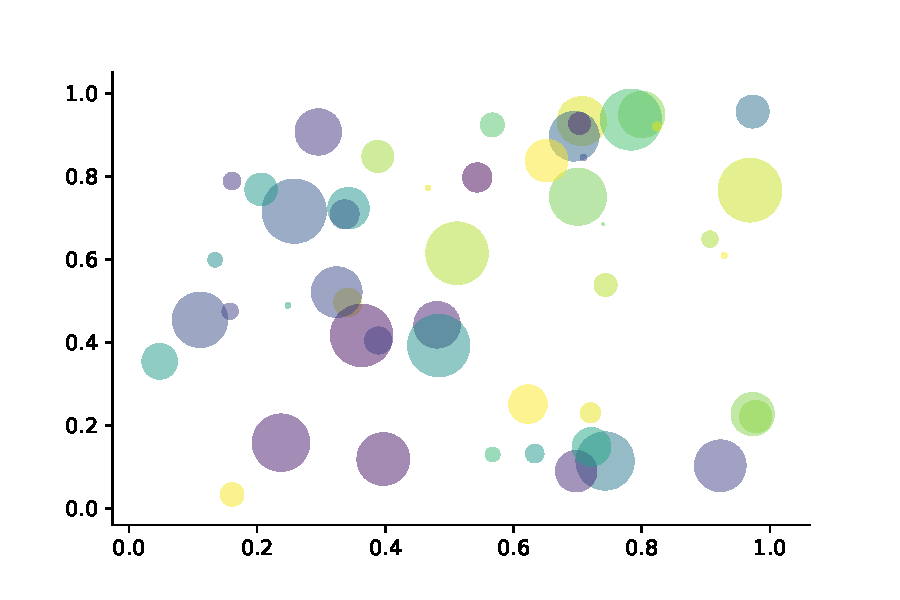
\includegraphics[width=0.6\textwidth]{scatter.pdf}
	\caption{Matplotlib: Scatter Plot Example\label{fig:mpg}}
\end{figure}


回归分析(regression analysis) 是确定两种或两种以上变量间相互依赖的定量关系的一种统计分析方法。根据定理~ \ref{thm:fubi},其运用十分广泛,回归分析按照涉及的变量的多少,分为一元回归和多元回归分析;按照因变量的多少,可分为简单回归分析和多重回归分析;按照自变量和因变量之间的关系类型,可分为线性回归分析和非线性回归分析。

但是由于绝对值不易作解析运算,因此,进一步用残差平方和函数来度量总偏差。偏差的平方和最小可以保证每个偏差都不会很大。于是问题归结为确定拟合函数中的常数和使残差平方和函数最小。
\begin{itemize}
	\item Routing and resource discovery;
	     \begin{itemize} 
      	   	\item Language Models
       	 	\item Vector Space Models
    		 \end{itemize}
	\item Resilient and scalable computer networks;
	\item Distributed storage and search.
\end{itemize}
\section{示例}
\begin{lstlisting}[frame=single]
\documentclass[geye,green,pad,cn]{elegantnote}

\title{Note Example}
\author{ddswhu}
\institute{Elegant\LaTeX{} Program}
\version{1.00}
\date{\today}

\begin{document}

\maketitle

\section{Introduction}
The content of Introduction.

\end{document}
\end{lstlisting}


\end{document}
